% Taken from Paper2 Basic research questions + experiments 1

\section{Experiment 1: Acceptance of AI Planning and PDDL Concepts}\label{sec:Exp1}

% \section{How do non-expert users adopt the automated planning language with its action model representation?}
%%%%%%%% 1.25 pages %%%%%%%
In this experiment, users were introduced to a symbolic planning language (a simplified version of PDDL), involving the STRIPS formalism with type structures (\sect{sec:AP})
Users were instructed to describe world state configurations to the robot.
The goal was to assess the user's adoption of the planning concepts (object types, properties, generalised properties, action models) and to verify that the symbolic planning language is appropriate for non-expert users.
\subsection{Experimental Setup \& Participants}
We recruited 10 participants (1 male, 9 female), who were Sociology students at Universit\'{e} Grenoble Alpes
3 participants reported no programming experience, 6  had experience with office productivity software (`beginner'), and 1 had previously taken a programming course before (`advanced').
%
The experimental setup consisted of a 2x2 board, 2 cubes, 1 ball, and 1 ball recipient.
%The experimenter showed the participants a video of the Baxter robot \cite{Baxter}
The participants were given sheets with empty tables to complete for each task
Each participant was allocated 1 hour, but the average duration of the experiment was 49 minutes.
The participants' behaviour was observed by the experimenter and recorded on camera. 

 
\subsection{Experimental Design \& Measurements}
%After a short introduction to the Baxter robot, 
Users were told that they needed to use a symbolic planning language, to describe the state of the world, and the semantic meaning of actions to the robot. 
Throughout the experiment, users were faced with three different scenarios. 
\fig{fig:scenarios-exp1} shows an example of the experimental design, where the robot's action was to move the ball to an occupied position (B2). 
We evaluated their capability, to apply the planning language to different situations.
The experiment consisted of the following phases:

\begin{figure}[t]
	\centering
	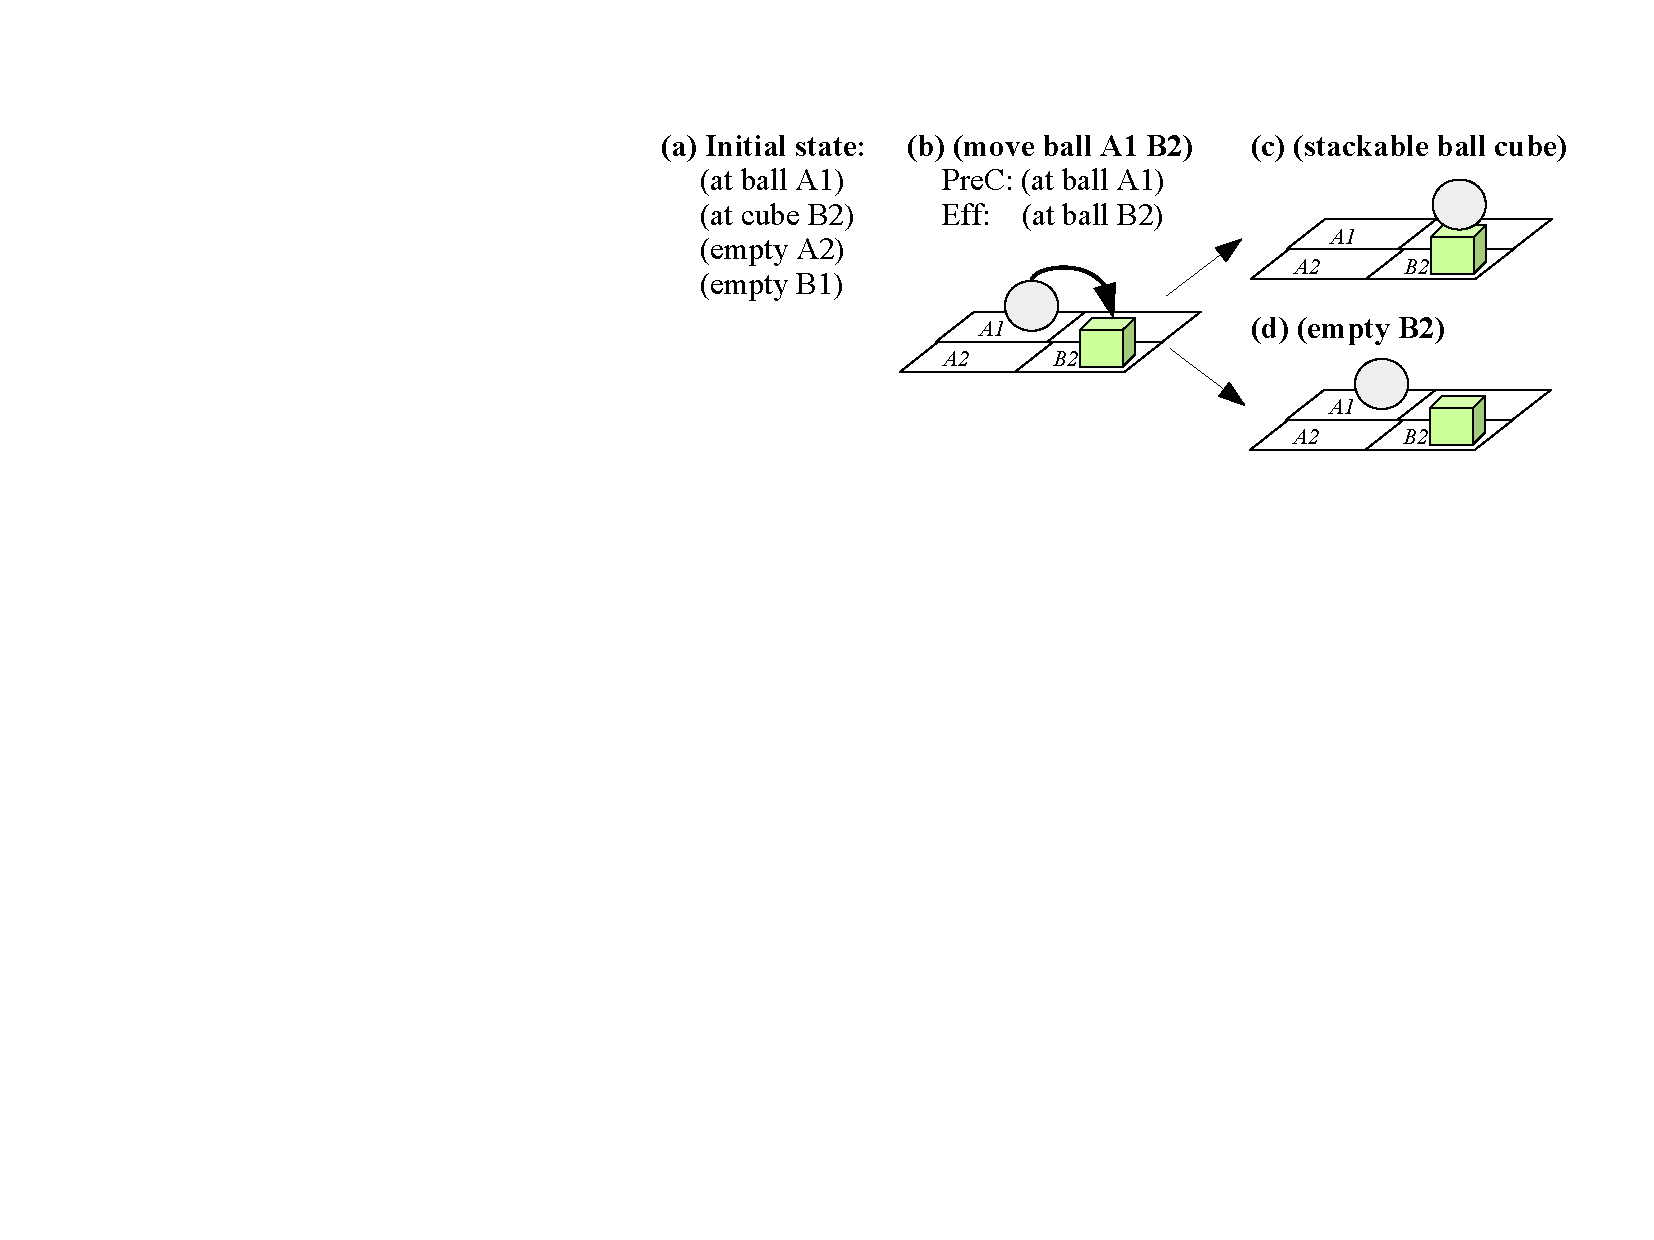
\includegraphics[width=0.75\linewidth]{figures/scenarios-exp1}
	\caption{Users were instructed to provide a description of (a) the initial state of the world and (b) an initial move action model
		They derived additional preconditions for moving the ball from position A1 to B2: (c) \textit{(stackable ball cube)}: the ball can be stacked onto the cube, and (d) \textit{(empty B2)}: if the ball cannot be stacked, the target position should be empty.}
	\label{fig:scenarios-exp1}
\end{figure}
\begin{itemize}
%  \item{Introduction: After a short introduction to the Baxter robot \cite{Baxter}, users were told that they needed to use a planning language (STRIPS) to explain Baxter the state of the world and the semantic meaning of the actions.}
  \item{\textbf{Training:} Users were presented with an initial world state and the symbolic planning language, to describe the object types and properties
Users were shown how to model a simple move action in terms of preconditions and effects (\fig{fig:action})
Additionally, they were introduced to the concept of \textit{generalised} properties and \textit{generalised} actions (\sect{sec:AP}).}
  \item{\textbf{Experimental test:} Users were presented a new world state and instructed to provide a description to the robot in the symbolic planning language (\fig{fig:scenarios-exp1}a)
After defining an initial move action model (\fig{fig:scenarios-exp1}b), users were faced with 3 different scenarios to refine the preconditions
Users derived a \texttt{(stackable ball cube)} property (\fig{fig:scenarios-exp1}c), which allowed a ball to be stacked on top of a cube
When this property did not hold, users proposed the \textit{empty} property (\fig{fig:scenarios-exp1}d), which the robot needed to verify before the action execution
At each step, users had to give the generalised representation of the properties and action models.}
  \item{\textbf{Planning:} Users were presented a description of a new state of the world and a goal state
Then, they had to define an action sequence, that allows the transition to the goal state (similar to \fig{fig:planning-permutation}c), and explain their reasoning using the symbolic action model representation.}
  \item{\textbf{Questionnaire:} Users were given a questionnaire containing 26 questions related to their experience, as well as their understanding of the learned planning language (\fig{fig:eEvaluation2}).}
   \item {\textbf{Debriefing:} Throughout the experiment, users were asked open-ended questions (``What properties do you observe in the current world state?"), so that they were guided as little as possible, and their responses were unbiased
When the participant struggled to find an answer, the experimenter guided the participant into a possible direction (``Why can the ball not be placed on the cube?").} 
\end{itemize}

\begin{figure}[ht]
	\centering
	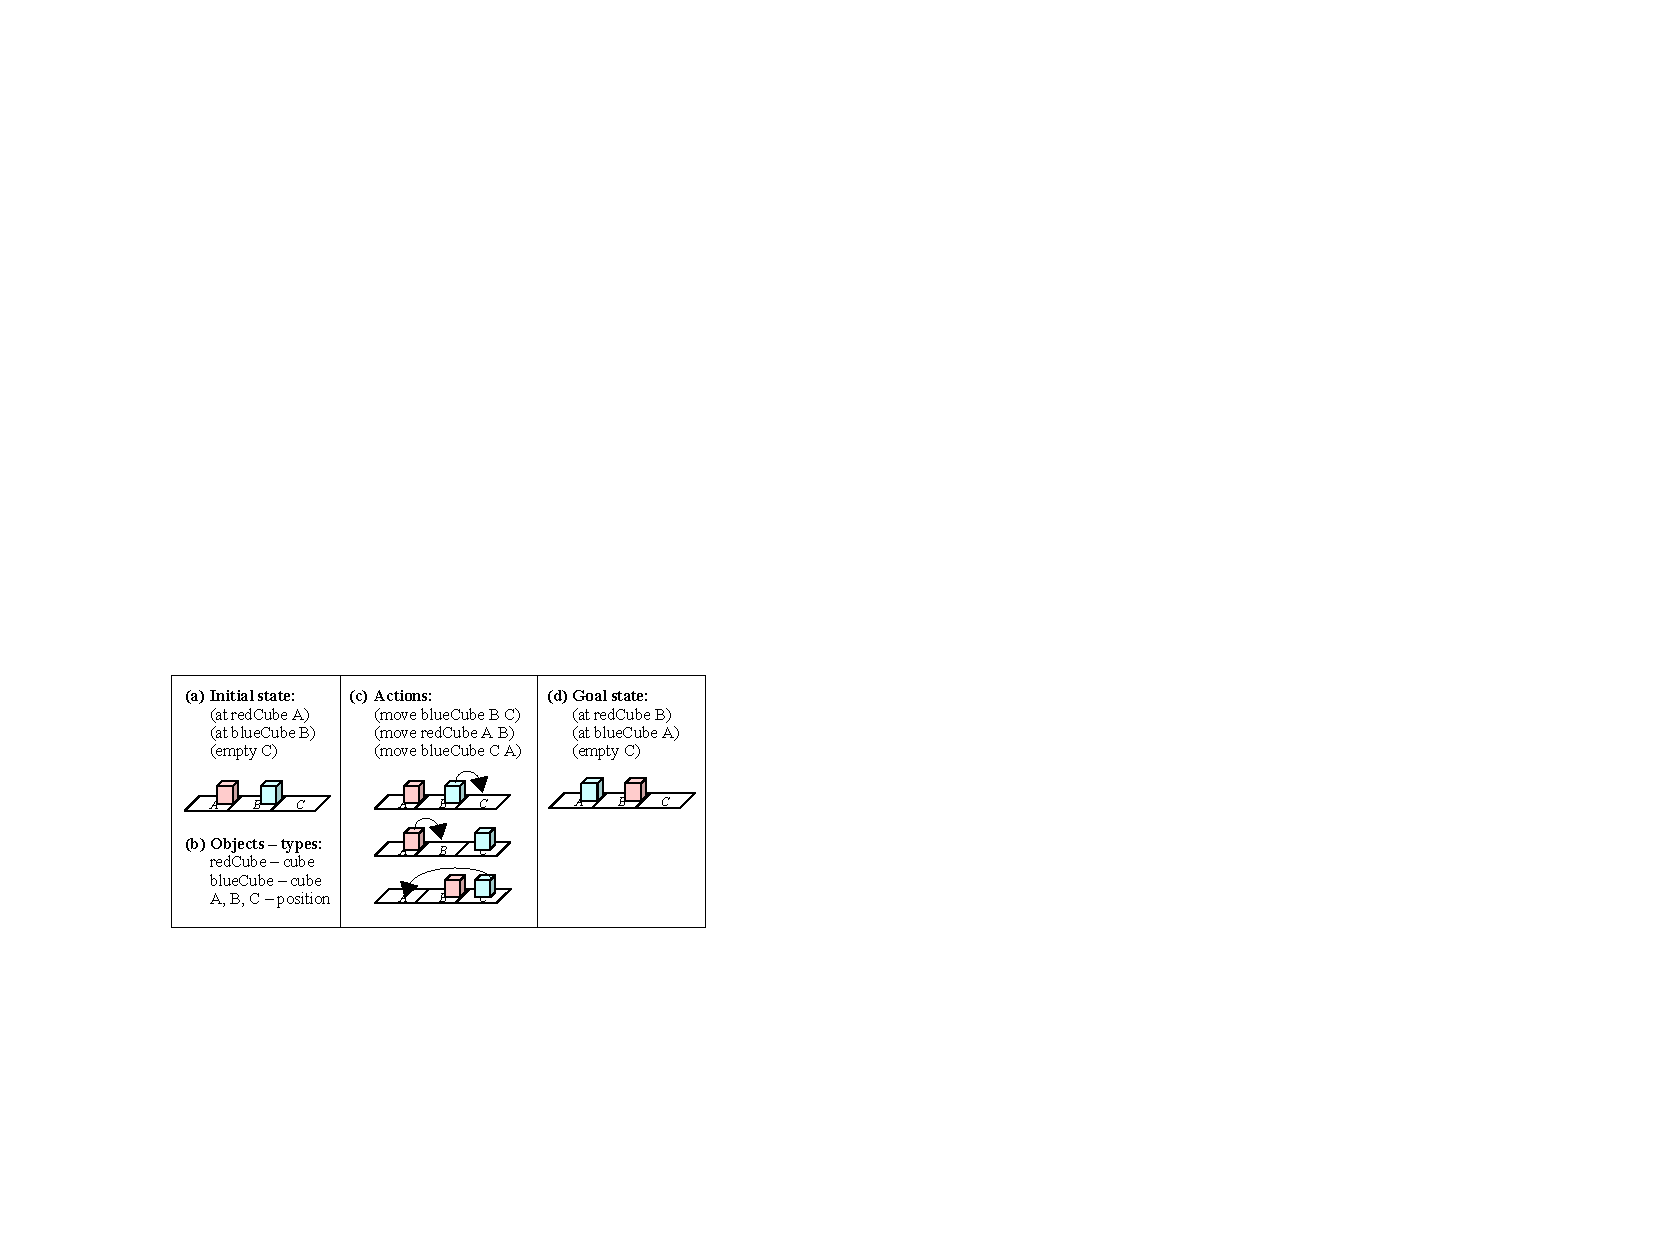
\includegraphics[width=0.8\linewidth]{figures/planning-permutation}
	\caption{Definition of a planning problem (a) properties describing the initial world state (b) object names and their types (c) instantiated actions (d) properties describing the goal state.}
	\label{fig:planning-permutation}
\end{figure}

\begin{figure}[ht]
	\centering
	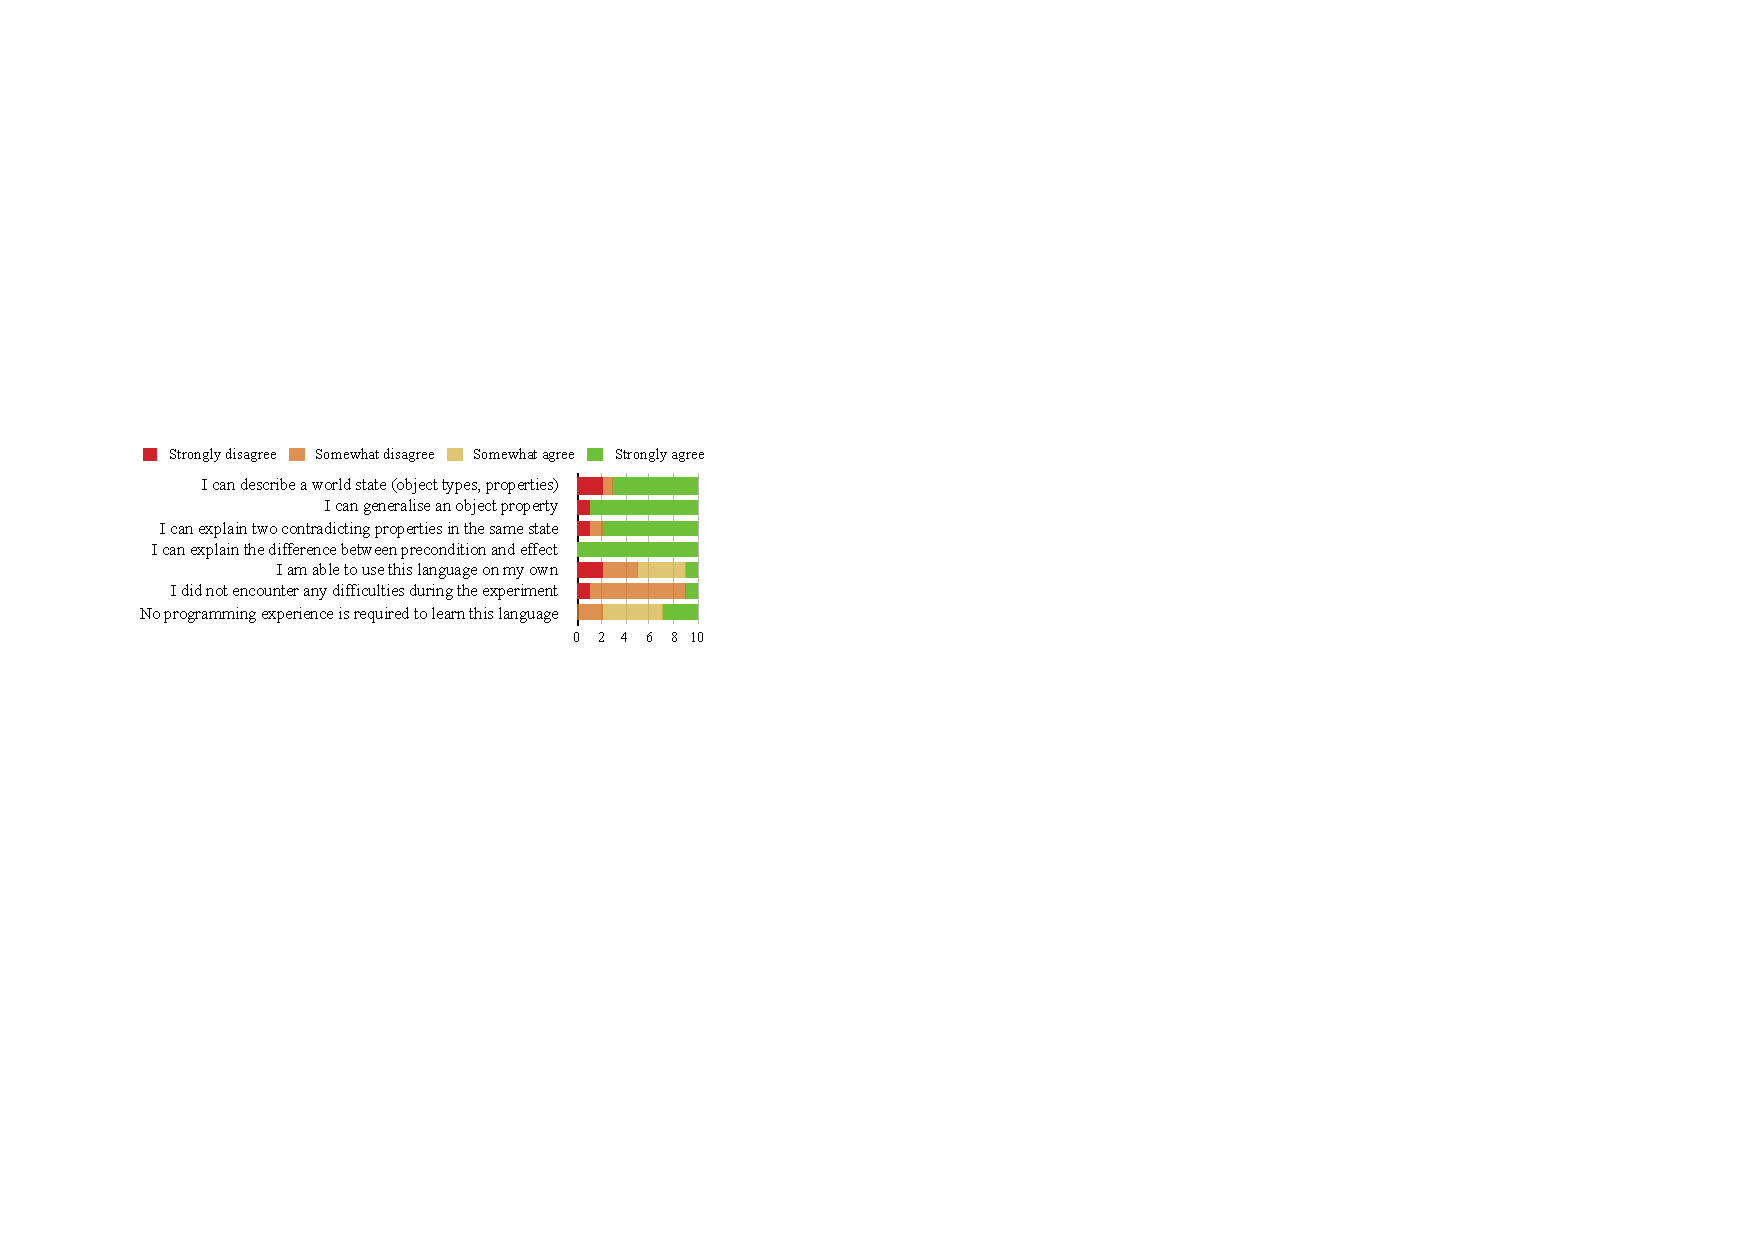
\includegraphics[width=0.85\linewidth]{figures/eEvaluation2}
	\caption{Summary of questionnaire responses: Extract of the 26 questions on the user's understanding, after the introduction to the automated planning language (\sect{sec:Exp1}).}
	\label{fig:eEvaluation2}
\end{figure} 

\subsection{Results}
We did not observe any significant differences in the performance of users with or without programming experience
9 (out of 10) participants found the symbolic representation of properties and actions easy to understand
During the experimental test, the majority (9) of the participants managed to describe the complete world state using the correct syntax.
When faced with different scenarios to refine the move action model, half of the participants struggled to formalise the \textit{stackable} condition in the symbolic language
They provided alternative formulations related to the cube's properties (``if the cube can hold the ball").
However, once the condition was defined, the majority (8) of the participants had little to no difficulties generalising this property.
Due to time constraints, only half (5) of the participants were presented the planning phase
All 5 encountered no problems when defining the action sequence to achieve the given goal.

In the questionnaire (\fig{fig:eEvaluation2}), the majority (9) of the participants understood the notion of states and object properties
8 correctly pointed out two properties that could not exist in the same state (e.g. \texttt{(empty A)} and \texttt{(at cube A)}).
All participants gave correct explanations for preconditions and effects of action models, and provided correct examples.
9 participants encountered difficulties during the experiment, 6 stated problems with formalising the language, especially at the beginning of the experiment.
Half of the participants believed that they could apply this language on their own.
No participants believed that an `expert' programmer was required to learn the symbolic planning language, but 7 participants believed that the minimum requirement was a `beginner' programming level, while 3 believed that no programming experience was required.

